\begin{ledgroupsized}[r]{120mm}
\footnotesize 
\pstart 
\noindent\textbf{\"{U}berlieferung:}
\pend
\end{ledgroupsized}
\begin{ledgroupsized}[r]{114mm}
\footnotesize 
\pstart \parindent -6mm
\makebox[6mm][l]{\textit{LiH}}%
Anstreichungen und Anmerkungen in \textsc{I.G. Pardies},\cite{00204} \textit{Discours du mouvement local}, Paris 1670: \textsc{Hannover}, GWLB,
 Leibn. Marg. 28. \pend
\end{ledgroupsized}

\vspace*{5mm}
\begin{ledgroup}
\footnotesize 
\pstart
\noindent\footnotesize{\textbf{Datierungsgr\"{u}nde:}
Leibniz verkehrte mit Pardies in Paris (siehe hierzu etwa \textit{LSB} II, 1 N.~133, S.~442; III,~1 N.~9, S.~42) und beschäftigte sich mit dessen mathematischen Werken eingehend während seines Pariser Aufenthaltes,
wie dies u.a. die Stücke \textit{LSB} VII, 3 N.~6, N.~26 und N.~38\textsubscript{12} belegen.
Die vorliegenden Marginalien dürften aber spätestens zu dem Zeitpunkt  verfasst worden sein, als Leibniz Pardies' \title{Statique} exzerpiert hat,
d.h. spätestens im Mai 1673 (siehe die Datierungsgründe in N.~7;
%= LH035_14_02_128v.tex + LH035_14_02_127r.tex = Aus und zu I. G. Pardies, La Statique
in N.~44
%= I. G. Pardies, La Statique = Pardies1673.tex
sind ferner Leibniz' Marginalien in seinem Handexemplar von \textit{La statique} ediert).
Denn wie Leibniz selbst zu Beginn von N.~7 referiert,
%= LH035_14_02_128v.tex + LH035_14_02_127r.tex = Aus und zu I. G. Pardies, La Statique
stellt Pardies seine \textit{Statique} als Fortsetzung des \title{Discours du mouvement local} dar
(siehe \cite{00296}\textsc{I.G. Pardies}, \textit{La statique}, Paris 1673, Préface).
%, S.~aij
Es erweist sich demgemäß als plausibel, die vorliegenden Marginalien auf den Zeitraum vom Frühjahr 1672 bis zum Mai 1673 zu datieren.}
\pend
\end{ledgroup}


\vspace*{8mm}
\pstart 
\normalsize
\noindent [Preface p. 1] PREFACE. / \textit{IE ne pretends pas faire ici l'eloge des Mechaniques} [...]\edtext{}{\lemma{}\Afootnote{\textit{Am oberen Rand rechts}: p. 13 negligit magnitudines corporum.\vspace{1mm}}}
\pend 
\count\Afootins=1200
\pstart  
[p. 29] Cequi est manifeste par les mesmes raisons que j'ai apport\'{e}es pour prouver que le mouvement dure to\^{u}jours. Mais il faut remarquer que lorsqu'vn corps a receu successivement plusieurs determinations differentes; il reste affect\'{e} de \edtext{la derniere}{\lemma{}\Afootnote{\textit{Leibniz unterstreicht}: la derniere, \textit{notiert daneben am Rand}: Error. Componuntur omnes in unum conatum \textit{und streicht schließlich die ganze Randbemerkung.}}}, sans que les precedentes fassent aucune impression sur lui.
\pend 
\pstart  
[p. 32] [...] ainsi le corps demeure affect\'{e} de la derniere determination: or cette derniere determination le portoit vers \textit{g}, c'est \`{a} dire qu'il faut prendre l'inclination qu'a la ligne courbe au point \textit{f}: et cette inclination se mesure par la tangente, comme s\c{c}avent les Geometres; ainsi c'est suivant cette tangente que le corps a\edtext{}{\lemma{}\Afootnote{\textit{Unter dem Text, gestrichen}: paralogismus
}} [p. 33] est\'{e} determin\'{e} pour la derniere fois; et par consequent c'est suivant cette ligne qu'il continu\"{e} de se mouvoir.
\pend 
\count\Afootins=1000
\pstart  
[p. 35] [...] tous ces corps continu\"{e}ront de se mouvoir en cercle, la boule \`{a} l'entour du clou o\`{u} elle est suspendu\"{e}: la rou\"{e} \`{a} l'entour de son essieu o\`{u} elle est attach\'{e}e: et la liqueur \`{a} l'entour du centre du vaisseau o\`{u} elle est renferm\'{e}e. De mesme si 
%HS: öffnende edtext-Klammer für Afn hierher versetzt
\edtext{deux corps estant attachez ensemble, sont \'{e}galement agitez vers des endroits differens; il faut necessairement que ces corps opposez se meuvent circulairement \`{a} l'entour du point qui est au milieu d'eux, et c'est}{\lemma{}\Afootnote{\textit{Leibniz unterstreicht}: si deux [...] d'eux, et c'est\vspace{1mm}}} [p. 36] ainsi qu'vn fuseau ou vne pirou\"{e}tte continu\"{e}nt de se mouvoir circulairement; parceque les parties oppos\'{e}es estant attach\'{e}es et vnies entre elles, et de plus estant meu\"{e}s par les doits, en deux sens differens, l'vne d'vn cost\'{e} l'autre de l'autre; il faut que ce fuseau se meuve \`{a} l'entour de soy mesme. Que si de plus ces parties oppos\'{e}es sont pouss\'{e}es in\'{e}galement, en sorte que l'vne soit port\'{e}e vn peu plus \edtext{v\^{i}te vers vn cost\'{e}: alors ce corps outre son mouvement circulaire \`{a} l'entour de soy-mesme, aura vn autre mouvement qui le portera tout entier sur quelques lignes differentes suivant la diversit\'{e} et la combinaison de ces determinations. Et c'est ainsi qu'vne pirou\"{e}tte d\'{e}crit}{\lemma{}\Afootnote{\textit{Leibniz markiert am Rand}: v\^{i}te vers vn cost\'{e} [...] qu'vne pirou\"{e}tte décrit \textit{und notiert}: \Denarius \hspace{1.8mm}Videtur eligi centrum propius parti victae quia si supponatur immobilis seu fixa ipsa erit centrum. Et tanto est propior immobili, quanto victa magis.}} par son essieu sur la table di[p. 36]verses figures entrelass\'{e}es tandis qu'elle se meut avec vne v\^{i}tesse incroyable \`{a} l'entour de son propre centre.
\pend 
\pstart  
[p. 39] [\textit{Gedruckte Marginalie}:] XVII. Dans la rencontre de deux corps il se fait vne \makebox[1.0\textwidth][s]{percussion, qui est mutuelle et \'{e}galement receu\"{e} dans l'vn et dans l'autre corps.}\\
\noindent [\textit{Haupttext}:] Or quoique bien souvent il n'y ait qu'vn corps qui\edtext{}{\lemma{}\Afootnote{\textit{Am Rand}: \Denarius}} se meuve et qui frappe,\hfill
tandis\hfill que\hfill l'autre\hfill demeure\hfill immobile\hfill et\hfill re\c{c}oit\hfill le\hfill coup;\hfill neanmoins\hfill la\hfill percussion\hfill est
\pend 
\vspace{1em}
\pstart
\centering
 \noindent 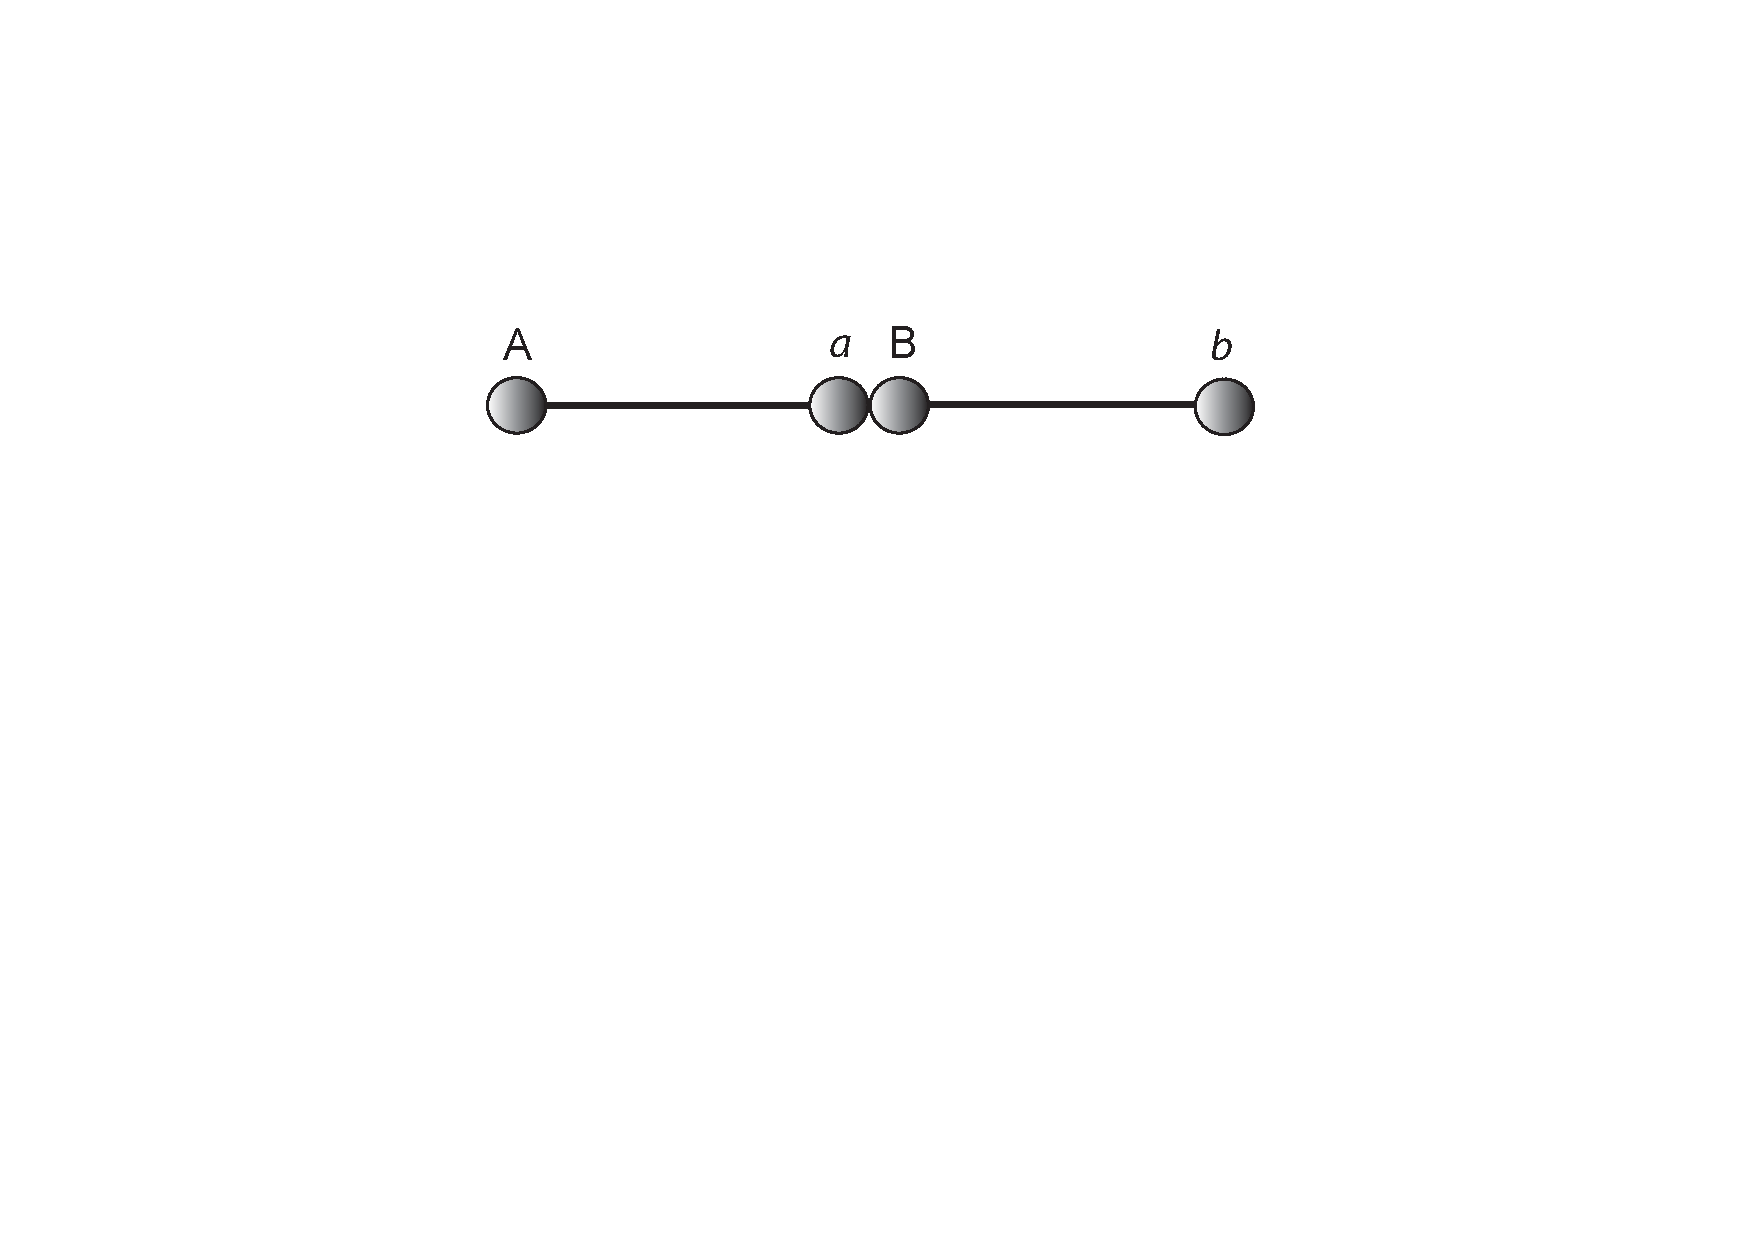
\includegraphics[trim = 0mm -3mm 0mm 0mm, clip, width=0.46\textwidth]{images/pardies1670-d1.pdf}\\
              \noindent \centering [\textit{Fig. 1}] 
\pend
\count\Afootins=1000
\pstart  
\noindent
to\^{u}jours mutuelle et elle est \'{e}galement receu\"{e} dans l'vn et dans l'autre corps: De sorte qu'autant que\edtext{}{\lemma{}\Afootnote{\hspace{1mm}\textit{Unter dem Text}: Il n'y a point de choc ny percussion sans resistance.}} [p. 40] le corps \textit{a} frappe le corps \textit{B}, autant est-il frapp\'{e} luy-mesme. \edtext{Ce que nous concevrons ais\'{e}ment si nous supposons que ces deux corps sont tout-\`{a}-fait semblables en masse, en figure, en}{\lemma{}\Afootnote{\hspace{-1mm}\textit{Leibniz markiert am Rand}: Ce que nous [...] en masse, en figure, en  \textit{und notiert}:
\Denarius}} duret\'{e}, et si de plus nous imaginons qu'ils aient du sentiment, et qu'ils soient capables de ressentir de la douleur quand ils sont frappez: [...]
\pend 
\count\Afootins=1000
\pstart  
[p. 41] Ainsi nous pouvons mettre pour vne maxime generale [p. 42] que \edtext{\textit{lorsque deux corps se frappent, la percussion est mutuelle et \'{e}gale de part et d'autre.}}{\lemma{}\Afootnote{\hspace{0.8mm}\textit{Neben dem kursiv gesetzten Text}: \Denarius}}
\pend 
\pstart  
[p. 42] Puis donc que la percussion que re\c{c}oit le corps \textit{B} est d'vn degr\'{e}, c'est \`{a} dire qu'elle est capable de porter le corps \textit{B} avec vn degr\'{e} de v\^{i}tesse
%HS: öffnende edtext-Klammer für Afn hierher versetzt
\edtext{vers \textit{b}; il faut aussi que la percussion que re\c{c}oit en mesme temps le corps \textit{a} soit aussi d'vn degr\'{e}; c'est \`{a} dire,}{\lemma{}\Afootnote{\hspace{0.8mm}\textit{Leibniz markiert am Rand}: vers \textit{b}; [...] c'est \`{a} dire  \textit{und notiert}:
error\vspace{1.1mm}}} qu'[p. 43]elle puisse porter le corps \textit{a} avec vn degr\'{e} de v\^{i}tesse vers les parties oppos\'{e}es, c'est \`{a} s\c{c}avoir vers \textit{A}.
\pend 
\vspace{1em}
\pstart
\centering
 \noindent 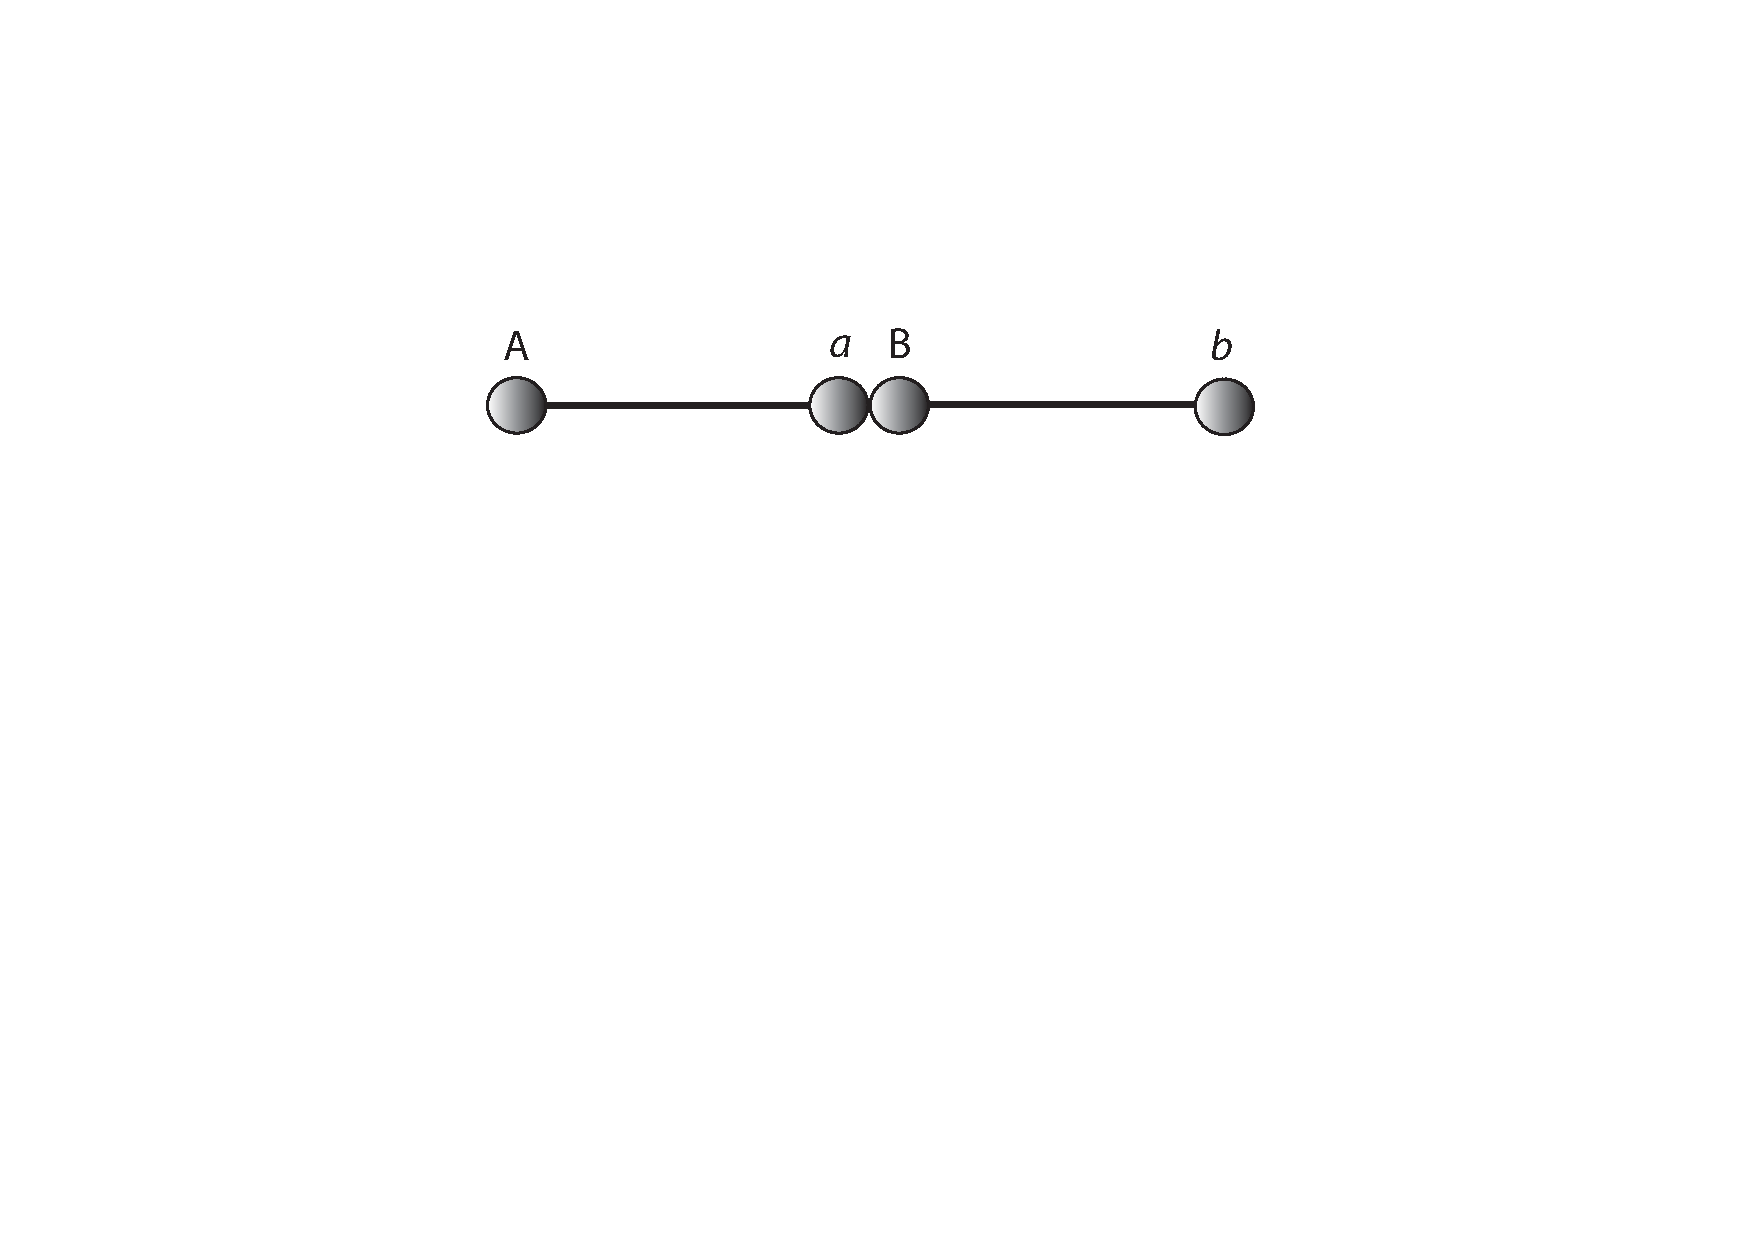
\includegraphics[trim = 0mm -3mm 0mm -5mm, clip, width=0.46\textwidth]{images/pardies1670-d2.pdf}\\
              \noindent \centering [\textit{Fig. 2}] 
\pend
\vspace{1em}
\pstart  
[p. 43] \setline{13}\edtext{Ainsi dans cette percussion le corps \textit{a} donne son mouvement et sa v\^{i}tesse au corps \textit{B}, et demeure cependant luy-mesme immobile.}{\lemma{}\Afootnote{\hspace{-1mm}\textit{Am Rand auf eingeklebtem Zettel}: Alia longe hujus rei ratio quaerenda, a natura pleni seu medii.\vspace{1mm}}}
\pend 
%\newpage
\count\Afootins=1200
\pstart  
[p. 46] D'o\`{u} l'on void encore que la percussion sera d'autant plus grande que cette approche mutuelle se sera plus viste. \edtext{De sorte que \textit{les percussions sont to\^{u}jours comme les v\^{i}tesses respectives}, pourveu que tout le reste soit pareil. Ainsi les deux corps s'approchant chacun}{\lemma{}\Afootnote{\textit{Am Rand auf eingeklebtem Zettel}: La veritable raison en est, parce qu'on peut dire, que
l'un est aussi bien meu vers l'autre, que l'autre vers luy.}} avec vn degr\'{e} de v\^{i}tesse absolu\"{e}, et faisant chacun vn pied de sa part dans vne minute; [...]
\pend 
\count\Afootins=1200
\pstart  
[p. 48] Estant donc certain que la percussion qui se fait en cette rencontre est de deux degrez; [\textit{Auf dieser H\"{o}he gedruckte Marginalie}:] XXI. \textit{Deux corps se mouvant l'vn vers l'autre rebroussent en faisant vn} \edtext{\textit{\'{e}change}}{\lemma{}\Afootnote{\hspace{1.8mm}\textit{Leibniz unterstreicht}: \'{e}change\textit{ und schreibt unter der gedruckten Marginalie}: \Denarius}} \textit{de leur vitesse}. [...]
\pend 
\pstart  
[p. 49] [...] d'vne de deux degrez vers \textit{A} qu'il re\c{c}oit dans la percussion, et d'vne autre d'vn degr\'{e} vers \textit{b}, qu'il avoit auparavant\edtext{}{\lemma{}\Afootnote{\hspace{1.8mm}\textit{Leibniz unterstreicht}: vers \textit{b}, qu'il avoit auparavant \textit{und notiert am Rand}: \Denarius}}; ainsi il luy reste seulement vn degr\'{e} libre d'impression et de v\^{i}tesse qui le porte vers \textit{A}. Et demesme \textit{B} sera port\'{e} vers \textit{b} avec vn degr\'{e} aussi de v\^{i}tesse; de fa\c{c}on que tous deux rebroussent sur la mesme ligne avec la mesme v\^{i}tesse qu'ils \edtext{sont venus}{\lemma{}\Afootnote{\hspace{1.8mm}\textit{Leibniz unterstreicht}: sont venus \textit{und notiert am Rand}: \Denarius}}. Que si nous supposons que l'vn s'avance plus v\^{i}te que l'autre; [...]
\pend 
\count\Afootins=1000
\pstart  
[p. 50] Que si les deux corps se meu[p. 51]vent
vers les mesmes endroits sur vne ligne droite, en sorte que le plus lent allant devant soit enfin \edtext{attrapp\'{e} par le plus v\^{i}te qui le suit}{\lemma{}\Afootnote{\hspace{-0.8mm}\textit{Leibniz unterstreicht}: attrapp\'{e} par le plus v\^{i}te qui le suit}}; alors tous les deux continueront de se mouvoir sur la mesme ligne vers les mesmes endroits; mais ils feront vn \'{e}change de leurs v\^{i}tesses\edtext{}{\lemma{}\Afootnote{\textit{Leibniz unterstreicht}: mais ils feront vn \'{e}change de leurs v\^{i}tesses.\vspace{1mm}}}. Soit le corps \textit{A} meu avec deux degrez de v\^{i}tesse \textit{b}, faisant dans vne minute deux pieds jusques en \textit{a}.
\pend 
\vspace{1em}
\begin{center}
 \noindent 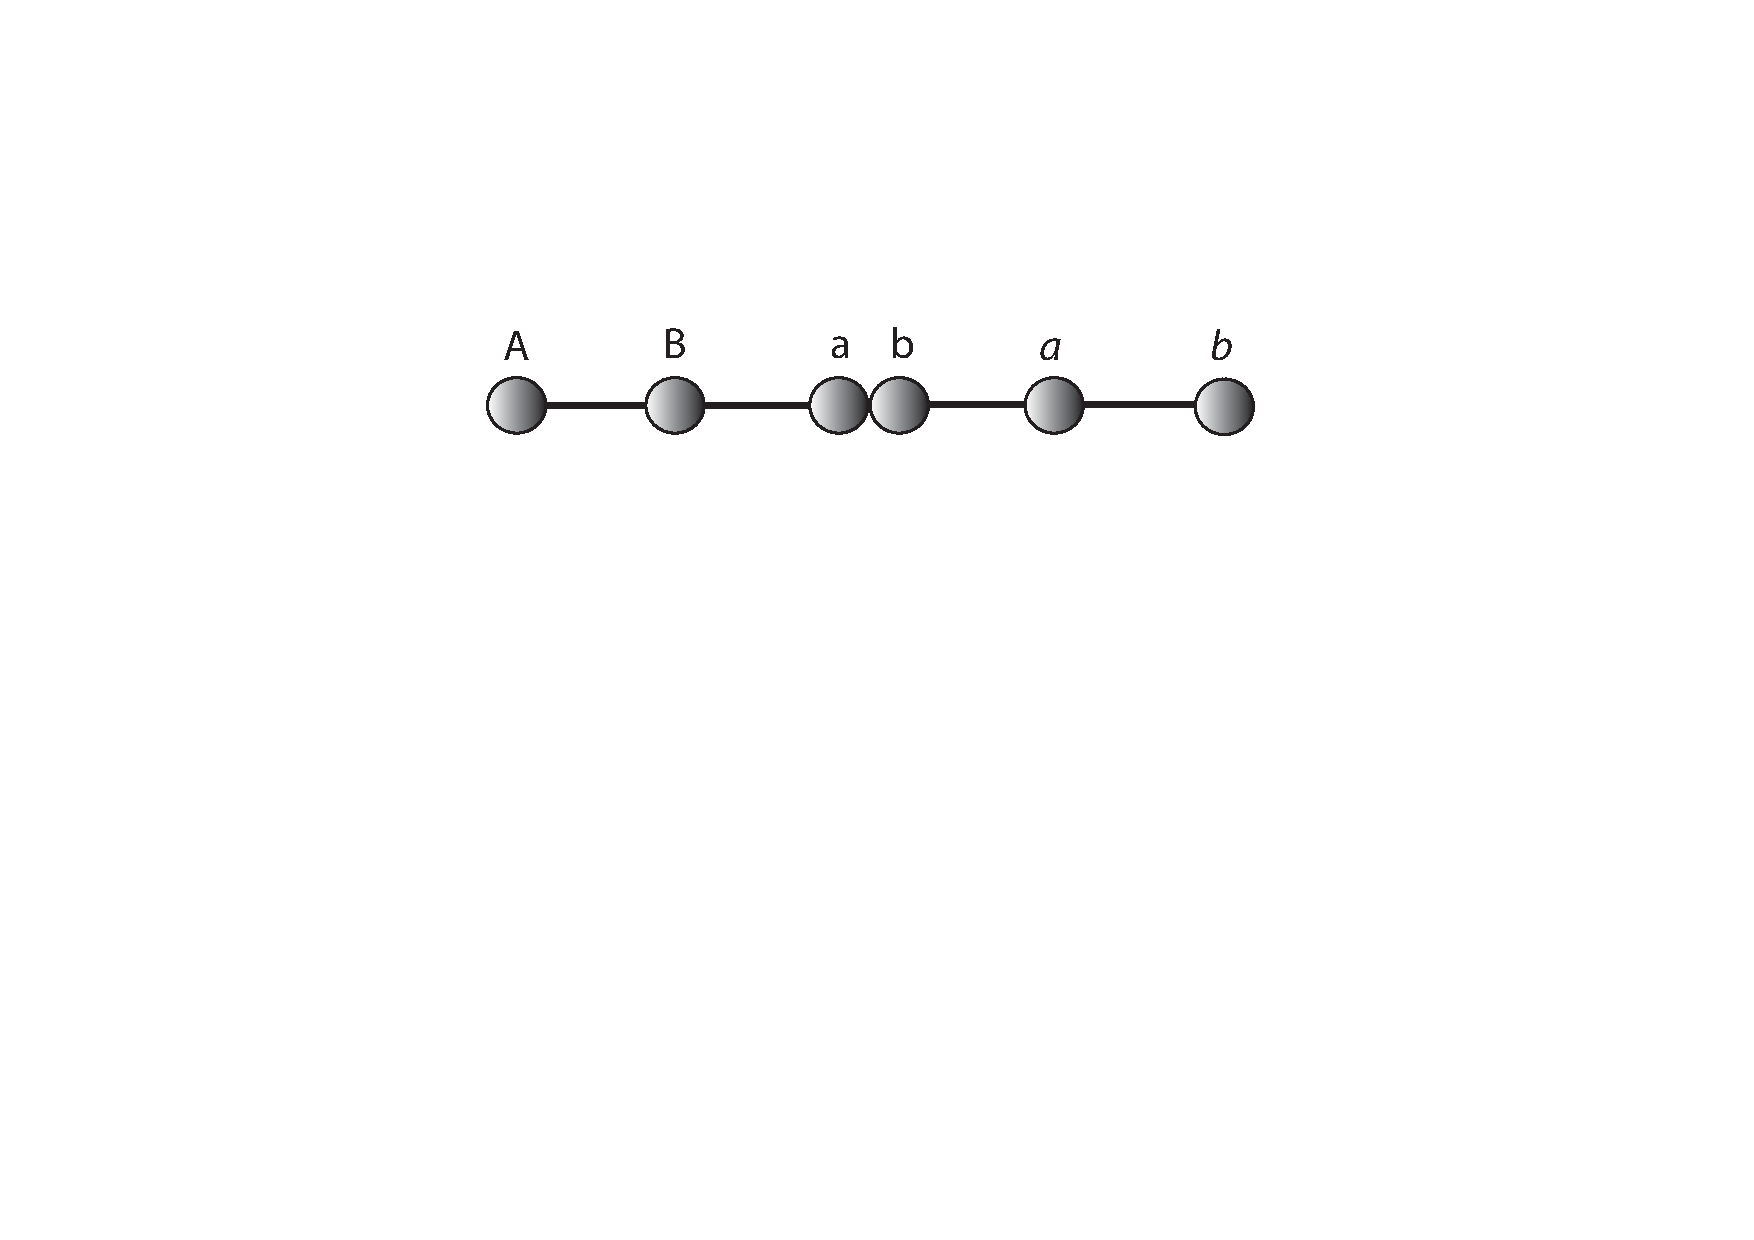
\includegraphics[trim = 0mm -3mm 0mm 0mm, clip, width=0.46\textwidth]{images/pardies1670-d3.pdf}\\
              \noindent \centering [\textit{Fig. 3}] 
\end{center}
\pstart  
[p. 53] \setline{15}Que si le corps qui est frapp\'{e} est tout-\`{a}-fait in\'{e}branlable; il faut voir quelle force aura la percussion, et ce que deviendra le corps qui frappe. [\textit{In dieser H\"{o}he gedruckte Marginalie}:] XXIII. \textit{Vn corps dur venant \`{a} frapper sur vn autre corps in\'{e}branlable, se refl\'{e}chit avec} \edtext{\textit{tout son mouvement.}}{\lemma{}\Afootnote{\textit{Leibniz unterstreicht}: tout son mouvement \textit{und schreibt unter der gedruckten Marginalie}: Il faut chercher d'autres raisons.}}
%diese Bfootnote erscheint nicht im Pdf, ich habe sie aus der Afootnote herausgenommen, verweist sie auf die richtige Stelle????
%{\lemma{chercher}\Bfootnote{\textit{(1)}\ des autres \textit{(2)}\ d'autres \textit{L}}} 
%HS: nachfolgende Bfn bleibt unterdrückt
%\edtext{}{\lemma{chercher}\Bfootnote{\textit{(1)}\ des autres \textit{(2)}\ d'autres \textit{L}}}
\pend
\count\Bfootins=1500
\pstart  
[p. 54] Mais si nous supposons qu'en mesme temps qu'\textit{A} vient frapper la lame en \textit{a}; en mesme temps aussi \textit{B} la vient frapper en \textit{b}; cette lame demeurera immobile, puisqu'elle est frapp\'{e}e \'{e}galement des deux costez opposez; et chaque corps rebroussera avec son degr\'{e} de v\^{i}tesse avec lequel il estoit venu. Car, comme j'ay dit, \edtext{ces deux corps se frappent nonobstant cette lame, comme s'il n'y avoit rien entre-deux}{\lemma{}\Afootnote{\textit{Leibniz unterstreicht}: ces deux [...] rien entre-deux\vspace{1mm}}}; or s'il n'y avoit rien entre-deux, ils rebrousseroient avec leur mesme degr\'{e} [p. 55] de v\^{i}tesse, comme il a est\'{e} prouv\'{e} au \S. 21. ainsi quoique cette lame se trouve l\`{a}; ils ne laisseront pas de rebrousser.
\pend 
\count\Afootins=1200
\pstart  
[p. 56] Et voil\`{a} comment on demonstre qu'vn corps dur venant \`{a} frapper vn autre corps dur inflexible et in\'{e}branlable, se refl\'{e}chit \edtext{avec tout son mouvement: ce que je ne pense pas que personne ait encore demonstr\'{e}.}{\lemma{}\Afootnote{\textit{Leibniz unterstreicht}: avec tout [...] encore demonstr\'{e} \textit{und notiert am Rand}: personne ait encore demonstr\'{e}.}}
\pend 
\pstart  
[p. 66] [...] parce-qu'alors la percussion seroit plus \edtext{droite: et en effet si l'on veut en faire le calcul (ce qui est fort ais\'{e} \`{a} faire sur celuy mesme qu'a fait c\'{e}t Auteur\protect\index{Namensregister}{\textso  {},}) on trouvera que l'obliquit\'{e} de ces mouvemens est to\^{u}jours toute telle qu'il faut pour faire la diversit\'{e} que nous voions dans les percussions d'vn corps qui tombe.}{\lemma{}\Afootnote{\textit{Leibniz markiert am Rand}: droite: et en effet [...] d'vn corps qui tombe.}}
\pend 
\pstart  
L'AUTRE remarque est sur ce que j'ay ve\^{u} dans quelques-vnes de nos citadelles, o\`{u} ceux qui les ont basties, \edtext{ont prefer\'{e} l'agr\'{e}emt des yeux \`{a} la force des}{\lemma{}\Afootnote{\hspace{-0.8mm}\textit{Leibniz unterstreicht}: ont prefer\'{e} l'agr\'{e}emt des yeux \`{a} la force des\vspace{1mm}}} murailles, lorsqu'au lieu de les faire tout-vnies, ils les ont diversifi\'{e}es de beaucoup d'ornemens de pierres qui avancent au dessus des autres: [...]
\pend 
%\newpage
\pstart  
[p. 67] Je dis que si toute cette variet\'{e} est agreable \`{a} la veu\"{e}; elle est aussi tres-desavantageuse pour la d\'{e}fense. \edtext{Car ces enfonceures et ces saillies de pierres donnent aux batteries obliques du canon le mesme avantage et la mesme force qu'ont les batteries droites. De-sorte que le boulet, qui}{\lemma{}\Afootnote{\hspace{-0.8mm}\textit{Leibniz markiert am Rand}: Car ces enfonceures [...] le boulet, qui \textit{und unterstreicht}: Car ces enfonceures [...] et la mesme}} venant de biais ne feroit qu'effleurer le mur s'il l'avoit trouv\'{e} tout plat; [...]
\pend 
\count\Afootins=1000
%\newpage
\pstart  
[p. 70] IL faut remarquer \edtext{qu'il n'est pas vrai qu'il y ait to\^{u}jours autant de mouvement absolu apr\'{e}s la percussion, qu'il y en a[p. 71]voit}{\lemma{}\Afootnote{\textit{Leibniz unterstreicht}: qu'il n'est pas vrai [...] qu'il y en avoit}} devant. Mais il est fort ais\'{e} \`{a} demonstrer \edtext{que le mouvement respectif est to\^{u}jours le mesme}{\lemma{}\Afootnote{\textit{Leibniz unterstreicht}: que le mouvement respectif est to\^{u}jours le mesme}}; en-sorte que les corps s'\'{e}loignent mutuellement l'vn de l'autre apr\'{e}s la percussion, aussi v\^{i}te qu'ils s'en approchoint devant.
\pend 
\pstart  
[p. 71] Et mesme apr\'{e}s que j'aurai expliqu\'{e} les mouvemens qui se font dans le plein; je croy qu'il me seroit facile, de prouver qu'ayant \'{e}gard generalement \`{a} tous les corps qui sont dans tout l'vnivers, \edtext{il y a presentement autant}{\lemma{}\Afootnote{\textit{Leibniz unterstreicht}: il y a presentement autant}} \edtext{de mouvement respectif, ni plus ni moins, qu'il y en avoit au commencement de la creation du monde}{\lemma{}\Afootnote{\hspace{-0.8mm}\textit{Leibniz markiert am Rand}: de mouvement respectif, [...] creation du monde.\vspace{1mm}}}.
\pend 
\count\Afootins=1000
\pstart  
[p. 72] Il est encore \`{a} remarquer que \edtext{le point du milieu}{\lemma{}\Afootnote{\textit{Leibniz unterstreicht}: le point du milieu \textit{und notiert hierzu}: Hugenii\protect\index{Namensregister}{\textso{Huygens}, Christiaan (1629-1695)} centrum gravitatis}} d'entre les deux corps se meut to\^{u}jours vniformement sur vne ligne droite, tirant sans aucune interruption vers les mesmes endroits.
\pend 
\count\Afootins=1000
\pstart  
[p. 72] On s'estonnera sans doute que dans toutes les regles precedentes je n'aye point fait mention de l'\'{e}galit\'{e} ou de l'in\'{e}galit\'{e} des corps qui se frappent. [p. 73] Et il semble d'abord qu'afin que ce que je viens de dire soit veritable it faut que je suppose que le corps sont parfaitement \'{e}gaux: [...] [\textit{Daneben gedruckte Marginalie:} p. 72] XXXI. \textit{Tout ces regles sont veritables, soit que les corps soient} [p. 73] \edtext{\textit{\'{e}geaux; soit qu'ils ne le soient pas.}}{\lemma{}\Afootnote{\textit{Leibniz markiert am Rand}: \textit{\'{e}gaux; soit qu'ils ne le soient pas.}}}
\pend 
\count\Afootins=1000
\pstart  
[p. 74] \edtext{Et si l'on y prend garde la force de la raison que j'ai apport\'{e}e au \S. 16. est to\^{u}jours la mesme}{\lemma{}\Afootnote{\textit{Am Rand und zwischen den Zeilen}: Error.\vspace{1mm}}} quoique les corps soient de differentes grandeurs. Car le corps frapp\'{e} estant tout-\`{a}-fait indifferent \`{a} demeurer en repos ou \`{a} prendre le mouvement, et tout l'effect de la percussion venant de l'impenetrabilit\'{e} des corps:
%diese Bfootnote erscheint nicht im Pdf, ich habe sie aus der Afootnote herausgenommen, verweist sie auf die richtige Stelle????
%HS: Bfn bleibt in dieser Form unterdrückt.
%\edtext{}{\lemma{Supponuntur d'autres}\Bfootnote{\textit{(1)}\ force \textit{(2)}\ vitesse \textit{L}}}
%HS: Bfn bezieht sich auf Afn/Marginalie und wird als Marginalienapparat wie folgt wiedergegeben (am besten am Ende der Seite, da aber die Umbrüche nicht feststehen vorerst direkt bei der entsprechenden Afn):
\edtext{}{\lemma{}\Afootnote{\hspace{0.8mm}\textit{Am Rand auf \"{u}berstehender Papierlasche}: Sans le mouuement dans un liquide il n'y auroit point de difference entre la\textsuperscript{[a]} vitesse absolue et respective, et par consequent ces regles precedentes ne reussiront pas.
\vspace{2mm}
\\
%Hier Marginalienapparat mit dem (korrigierten) Text der Bfn:
\footnotesize
\textsuperscript{[a]} la\ \textit{(1)}\  force \textit{(2)}\ vitesse \textit{L}\vspace{1mm}}} 
%HS: Bfn bleibt in dieser Form unterdrückt.
%\edtext{}{\lemma{Supponuntur d'autres}\Bfootnote{\textit{(1)}\ force \textit{(2)}\ vitesse \textit{L}}}
si nous supposons que le corps frapp\'{e} soit plus grand, pourveu que toutes ses parties soient bien vnies ensemble, il faudra qu'il se meuve de la mesme v\^{i}tesse que se meut le corps qui frappe, [...]
\pend 
\count\Afootins=1200
\pstart 
[p. 76] Si cette substance est parfaitement fluide, c'est-\`{a}-dire si toutes ses parties, aussi bien les petites que les grandes, sont flexibles et liquides: [...] [\textit{Daneben gedruckte Marginalie}:] XXXII. \textit{Vn corps se meut dans le plein, aussi librement que dans le vuide.}\edtext{}{\lemma{}\Afootnote{\textit{Leibniz markiert am Rand die gesamte gedruckte Marginalie.\vspace{1mm}}}}
\pend 
\pstart  
[p. 77] [...] mais ces parties de la liqueur estant pouss\'{e}es, en poussent d'autres; et ainsi \edtext{jusqu'\`{a} l'extremit\'{e}}{\lemma{}\Afootnote{\textit{Leibniz unterstreicht}: jusqu'\`{a} l'extremit\'{e}, \textit{und notiert am Rand}: Hoc nihil est. Exiguum circulum faciunt tantum.\vspace{1mm}}}, d'o\`{u} il se fait vne reflexion par laquelle les parties qui se trouvent apr\'{e}s le corps dur, sont pouss\'{e}es avec la mesme force pour suivre ce mesme corps.
\pend 
\pstart  
[p. 78] [...] il n'est pas possible que les parties qui devancent le corps se meuvent sans que les parties qui suivent le mesme corps ne se meuvent aussi avec la mesme force. Ainsi autant que le corps dur \edtext{est retard\'{e}}{\lemma{}\Afootnote{\textit{Leibniz unterstreicht}: est retard\'{e} \textit{und notiert am Rand}: Pourquoy dans l'hypothese de l'auteur ils ne doivent point retarder, puisque la grandeur ny fait rien.\vspace{-0.5mm}}} par les parties qui le precedent, autant est-il repouss\'{e} par celles qui le suivent, et par consequent si le mouvement a vne fois commenc\'{e}, il doit continuer comme si c'estoit dans le vuide.
\pend 
\pstart  
[p. 79] [...] la communication de l'impression ne se peut faire parfaitement, et ainsi les parties posterieures de la liqueur ne seront pas tant pouss\'{e}es que les anterieures, et par consequent ne pousseront pas tant le corps dur, que celles de devant \edtext{le retardent}{\lemma{}\Afootnote{\hspace{-1.8mm}\textit{Leibniz unterstreicht}: le retardent.\vspace{1mm}}}. Et c'est pour cette raison que tous nos mouvements cessent [...]
%\edtext{}{\lemma{entre la}\Bfootnote{\textit{(1)} force \textit{ (2) } vitesse \textit{L}}}
\pend 
%\newpage
\count\Afootins=1200
\pstart  
[p. 82\,f.] [\textit{gedruckte Marginalie}:] XXXV. \edtext{\textit{Lorsque les corps sont in\'{e}gaux, les percussions se font dans le plein autrement que dans le vuide}}{\lemma{}\Afootnote{\textit{Leibniz markiert am Rand die gedruckte Marginalie und notiert darunter}: Je doute fort que le plein en repos differe du vuide.}}. [\textit{Haupttext}:] Mais si le corps frappant est plus grand, il faut necessairement qu'il ne re\c{c}oive pas tant d'effet de la percussion que l'autre, parcequ'il est emport\'{e} avec plus de violence par la liqueur qui l'environne; car nous voions qu'vne poutre emport\'{e}e par le [p. 83] courant d'vne riviere a bien plus d'effet quand elle vient \`{a} heurter contre vn pont ou contre vn moulin, que n'auroit\hfill pas\hfill vn\hfill b\^{a}ton\hfill emport\'{e}\hfill aussi\hfill par\hfill la\hfill mesme\hfill riviere;\hfill quoique\hfill d'ailleurs\hfill la\hfill poutre
\pend
\newpage
\pstart \noindent n'allast pas plus v\^{i}te que le b\^{a}ton: \edtext{et cela parce que la poutre venant \`{a} heurter est encore pouss\'{e}e par la grande quantit\'{e} d'eau qui l'environne, au-lieu que le b\^{a}ton l'est fort peu \`{a} cause du peu de place qu'il occupe et du peu d'eau dont il est emport\'{e}. Ainsi donc si le petit corps est en repos et que le grand vienne \`{a} le}{\lemma{}\Afootnote{\textit{Am Rand}: Si la poutre n'avoit qu'une petite base de la grandeur d'un baston, qui la so\^{u}tiendroit dans l'eau le m\^{e}me arriveroit. Ce n'est donc pas la grandeur de l'eau qui le pousse mais sa propre.}} frapper; [...]
\pend 
\pstart  
[p. 84] Au-contraire si le grand est en repos, le plus petit apr\'{e}s avoir frapp\'{e} l'autre et luy avoir communiqu\'{e} vne partie de son mouvement, se refl\'{e}chira en perdant vne partie de sa v\^{i}tesse. Et de tout ceci il paroist \edtext{qu'Aristote n'est pas si blasmable}{\lemma{}\Afootnote{\textit{Leibniz unterstreicht}: qu'Aristote n'est pas si blasmable}} que quelques-vns pretendent, lorsque pour expliquer les causes de la continuation des mouvemens que nous voions, il a emploi\'{e} le \textit{medium}, c'est-\`{a}-dire la substance liquide dans laquelle nos corps se meuvent.
\pend 
\count\Afootins=1200
\count\Cfootins=1200
\pstart  
[p. 85] [...] de la facilit\'{e} qu'ils ont de se condenser ou de se rarefier, et de beaucoup d'autres choses qui ne peuvent nous estre connu\"{e}s non plus qu'vne infinit\'{e} d'autres empeschemens dont les combinaisons peuvent diversifier infiniment tous les effets des percussions. Seulement je \edtext{puis dire qu'en faisant vne certaine hypothese, qui paroist assez naturelle, on peut faire voir par les regles precedentes, que les percussions des corps in\'{e}gaux se feront de la maniere que veut Monsieur Hugens\protect\index{Namensregister}{\textso {Huygens}, Christiaan (1629-1695)} dans le dernier \textit{\edtext{Journal des S\c{c}avans.}{\lemma{Journal des S\c{c}avans}\Cfootnote{\cite{01118}\textsc{C. Huygens}, \glqq Extrait d'une lettre à l'auteur du Journal\grqq, \title{JS}, 18.~März 1669, S.~22-24 (\cite{00113}\title{HO} VI, S.~383-386).}}} Mais je ne veux pas m'ar}{\lemma{}\Afootnote{\textit{Leibniz markiert am Rand}: puis dire qu'en [...] je ne veux pas}}[p. 86]\edtext{rester l\`{a} davantage, peut-estre trouverai-je en quelque autre}{\lemma{}\Afootnote{\textit{Am Rand}: pourquoy non icy.}} rencontre occasion d'en parler plus amplement.
\pend 
\count\Cfootins=1500
%\newpage
\pstart  
[p. 87] Je ne veux pas marquer les mesures de ces refractions, parce que cela a est\'{e} fait par d'autres, et que leurs demonstrations se peuvent fort bien accommoder avec les choses que j'ai ici avanc\'{e}es. Je ne parle pas non plus ici de la refraction de \edtext{la lumiere}{\lemma{}\Afootnote{\textit{Leibniz unterstreicht}: la lumiere}}, parce que je croi qu'elle se fait tout autrement, \edtext{c'est-\`{a}-dire par des causes et des moiens tout differens}{\lemma{}\Afootnote{\textit{Leibniz unterstreicht}: c'est-\`{a}-dire par des causes et des moiens tout differens}}, comme je pourrois faire voir si je faisois quelques [p. 88] autres discours du mouvement.
\pend 
%\newpage
\pstart  
[p. 88] Il faudroit encore parler du mouvement des liqueurs, tant de leur chute que de leur faillie, comme aussi de leurs ondulations et de choses semblables: mais tout cela merite autant de discours particuliers. Et \edtext{comme je croy avoir trouv\'{e} quelque chose de nouveau sur ces matieres, je ne feray point}{\lemma{}\Afootnote{\textit{Leibniz markiert am Rand}: comme je croy [...] je ne feray point}} difficult\'{e}, de donner au public mes pens\'{e}es \`{a} examiner, si je voi que ce premier dis[p. 89]cours n'ait pas est\'{e} jug\'{e} tout-\`{a}-fait indigne d'estre le\^{u} par les personnes qui se plaisent \`{a} de semblables matieres.
\pend 
\count\Afootins=1200
%\newpage
\pstart  
[p. 98] \textit{Ie vous dis dernierement lorsque nous estions ensemble, non pas \`{a} la verit\'{e} que la lumiere se mouvoit en vn instant, comme vous m'\'{e}crivez; mais (ce que vous croyez estre la mesme chose) que du corps lumineux elle parvenoit en vn instant jusqu'\`{a} nos yeux: et mesme j'ajo\^{u}tai que je pensois s\c{c}avoir cela si certainement,} \edtext{\textit{que si on me pouvoit convaincre de fausset\'{e} l\`{a}-dessus, j'estois tout prest d'avouer que je ne s\c{c}avois rien du tout en Philosophie. Et vous au contraire, vous assuriez que la}}{\lemma{}\Afootnote{\textit{Leibniz markiert am Rand}: \textit{si on me pouvoit} [...] \textit{vous assuriez que la}}} \textit{lumiere ne se mouvoit pas en vn instant; et vous disiez avoir trouv\'{e} vn moyen d'en faire l'experience, par lequel il seroit ais\'{e} devoir} [p. 99] \textit{qui de nous deux se trompoit en cela.}
\pend 
\pstart 
[p. 99] \edtext{\textit{Si quelqu'vn portant de nuit vn flambeau \`{a} la main, et le faisant mouvoir, jette la veu\"{e} sur vn miroir \'{e}loign\'{e} de luy d'vn quart de lieu\"{e}, il pourra tres-ais\'{e}ment remarquer, s'il sentira le mouvement qui se fait en sa main, auparavant que de le voir par le moyen du miroir.}}{\lemma{}\Afootnote{\textit{Leibniz markiert am Rand}: Si quelqu'vn [...] le moyen du miroir.}} \textit{Et vous vous assuriez tellement sur cette experience, que vous estiez prest de croire que toute vostre Philosophie estoit fausse,} [...]
\pend 
\count\Afootins=1200
%\newpage
\pstart  
[p. 118] Ainsi la lumiere qui est maintenant parvenu\"{e} \`{a} nous, estant sortie de C, o\`{u} estoit la Lune demi-heure auparavant, nous doit faire voir la Lune en \edtext{E}{\lemma{}\Afootnote{\textit{Leibniz ersetzt} E \textit{durch} C.}}, en quelque part du monde qu'elle se puisse maintenant trouver, quand elle seroit demeur\'{e}e immobile, ou qu'elle auroit est\'{e} transport\'{e}e: [...]
\pend 
\pstart  [p. 146] M. Descartes se sert tres-mal du principe qui a est\'{e} expliqu\'{e} 
\edtext{au \S. 13.}{\lemma{au \S. 13.}\Cfootnote{\textsc{I. G. Pardies},\cite{00204} \textit{Discours du mouvement local}, Paris, 1670, S. 33.}} 
\edtext{\textit{Que tout corps qui se meut autour d'vn centre, fait effort pour s'en \'{e}loigner.} On peut faire voir qu'il s'est tromp\'{e} en}{\lemma{}\Afootnote{\hspace{-1.3mm}\textit{Leibniz markiert am Rand}: \textit{Que tout corps} [...] s'est tromp\'{e} en\vspace{1mm}}} [p. 147] voulant expliquer par l\`{a} la pesanteur des corps. Aussi ne pretend-on pas donner \`{a} ce principe toute l'\'{e}tendu\"{e} que luy donne M. Descartes.
\pend 
\pstart  [p. 147] L'auteur de ce discours est pleinement persuad\'{e}, que quand bien il n'y auroit point de saintes Ecritures, l'hypothe[p. 148]\edtext{se qui met la terre immobile, est preferable \`{a} toute autre.}{\lemma{}\Afootnote{\textit{Leibniz unterstreicht und markiert am Rand}: qui met la terre immobile, est preferable \`{a} toute autre.}} On a seulement voulu faire voir que c\'{e}t argument n'est pas convainquant: il y en a d'autres qui sont meilleurs, sur tout celuy qui a est\'{e} fait valoir en de fort belles occasions; pris du mouvement \edtext{tonique}{\lemma{}\Afootnote{\textit{Leibniz unterstreicht}: tonique}} de l'aiman.
\pend
 \count\Afootins=1500
 \count\Bfootins=1500
 \count\Cfootins=1500

